\bluepage{Advanced Draw Calls}

\begin{frame}[fragile]
\frametitle{Advanced draw commands}
	\begin{itemize}
	\item There is a lot of variants of following commands:
\begin{minted}[bgcolor=bg]{packages/c_cpp.py:CppLexer -x}
glDrawArrays glDrawElements
\end{minted}
	\item Instancing
	\item Indirect Draw
  \item Multi Draw
	\end{itemize}
{\tiny
\begin{minted}[bgcolor=bg]{packages/c_cpp.py:CppLexer -x}
glDrawArrays,glMultiDrawArrays

glDrawArraysInstanced,glDrawArraysInstancedBaseInstance,

glDrawArraysIndirect,glMultiDrawArraysIndirect

glDrawElements,glDrawRangeElements,glMultiDrawElements

glDrawElementsBaseVertex,glDrawRangeElementsBaseVertex,glMultiDrawElementsBaseVertex
glDrawElementsInstanced,glDrawElementsInstancedBaseInstance,glDrawElementsInstancedBaseVertex, 
glDrawElementsInstancedBaseVertexBaseInstance

glDrawElementsIndirect,glMultiDrawElementsIndirect
\end{minted}
}
\end{frame}

\begin{frame}[fragile]
\frametitle{Advanced draw commands - instancing}
	\begin{figure}[h]
	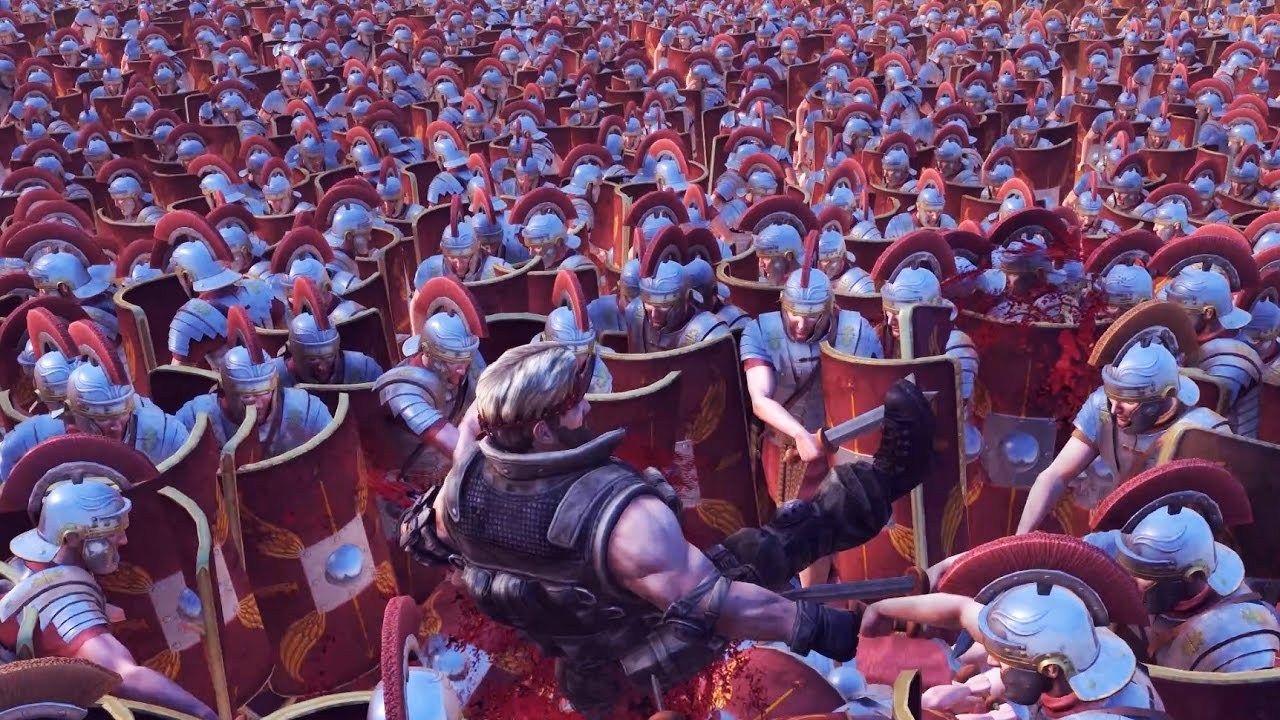
\includegraphics[width=10cm,keepaspectratio]{pics/uebs_instancing.jpg}
	\end{figure}
\url{http://epicbattles.wikia.com/wiki/File:UEBS_Chunk.jpg}
\end{frame}

\begin{frame}[fragile]
\frametitle{Advanced draw commands - instancing}
	\begin{itemize}
	\item Instancing draws same mesh in multiple instances, each with different transformation matrix.
	\item Instance id can be access in shader through built-in variable: gl\_InstanceID
	\item Instance id can be used as index into array of transformation matrices or materials.
	\end{itemize}
{\scriptsize
\begin{minted}[bgcolor=bg]{packages/graphics.py:GLShaderLexer -x}
#version 460

layout(location=0)in vec4 Position;
uniform mat4 MVP[100];

void main(){
  gl_Position=MVP[gl_InstanceID]*Position;
}
\end{minted}
}
{\scriptsize
\begin{minted}[bgcolor=bg]{packages/c_cpp.py:CppLexer -x}
glBindVertexArray(VAO);
glDrawArraysInstanced(GL_TRIANGLES,0,NumVertices,NumInstances);
glBindVertexArray(0);
\end{minted}
}
\end{frame}

\begin{frame}[fragile]
\frametitle{Advanced draw commands - indirect calls}
	\begin{figure}[h]
	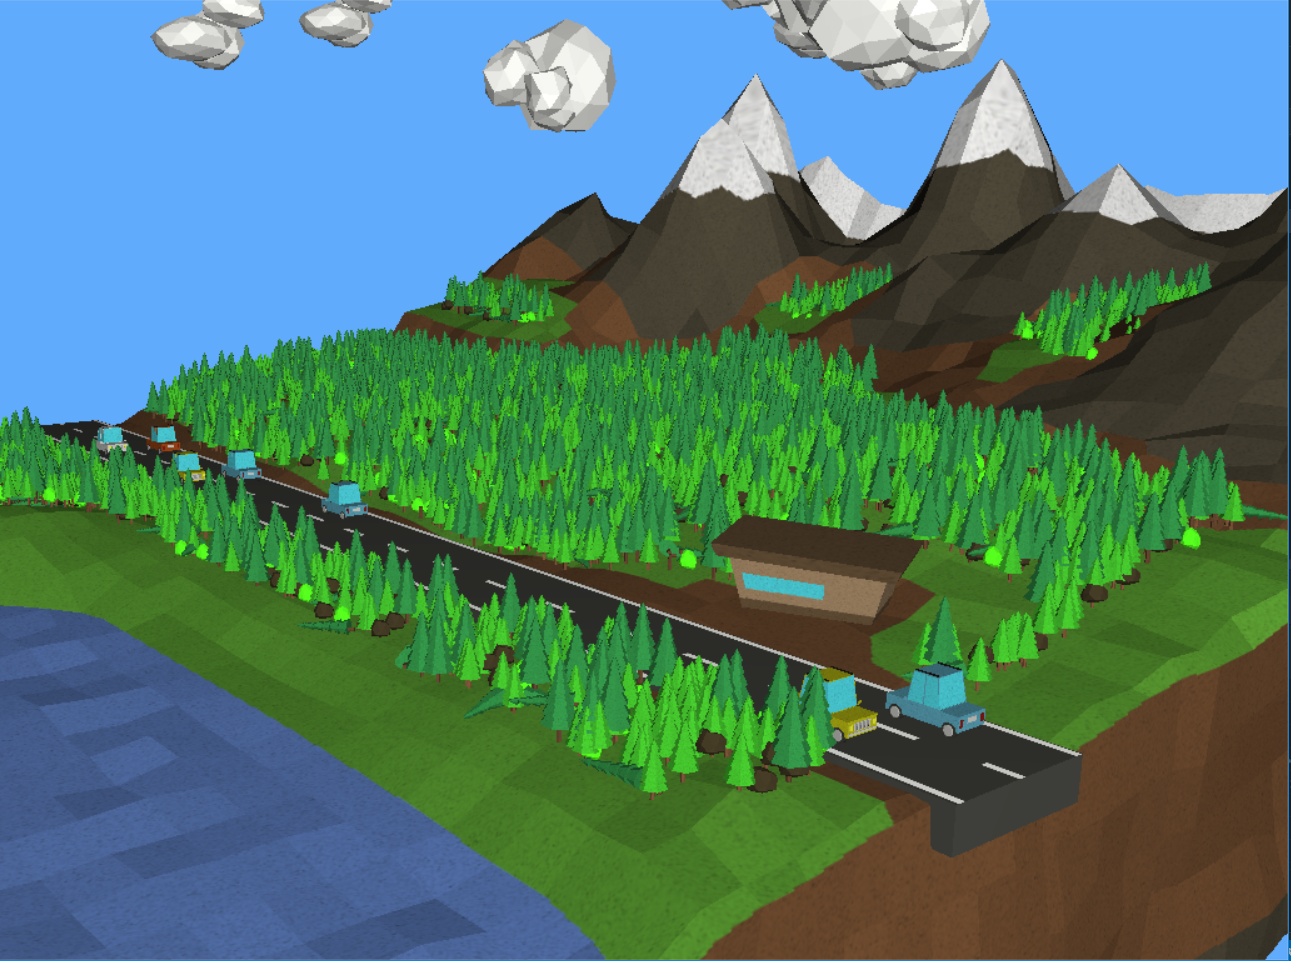
\includegraphics[width=10cm,keepaspectratio]{pics/indirect.png}
	\end{figure}
\url{http://www.fit.vutbr.cz/study/DP/DP.php.cs?id=18392&file=t}
\end{frame}

\begin{frame}[fragile]
\frametitle{Advanced draw commands - indirect draw calls}
	\begin{itemize}
  \item Draw call can be stored in buffers.
  \item There is no need for CPU synchronization.
  \item It can be combined with compute shader, atomic counters, transform feedback, ...
	\end{itemize}
{\scriptsize
\begin{minted}[bgcolor=bg]{packages/c_cpp.py:CppLexer -x}
//init
glGenBuffers(1,&IndirectBuffer);
glBindBuffer(GL_DRAW_INDIRECT_BUFFER,IndirectBuffer);
unsigned Data[4]={100,1,0,0};//command
glBufferData(GL_DRAW_INDIRECT_BUFFER,sizeof(unsigned)*4,
  Data,GL_DYNAMIC_DRAW);

//...
//fill buffer from GPU
//...

//draw
glBindBuffer(GL_DRAW_INDIRECT_BUFFER,IndirectBuffer);
glDrawArraysIndirect(GL_TRIANGLES,NULL);
\end{minted}
}
\end{frame}

\begin{frame}[fragile]
\frametitle{Advanced draw commands - multi draw calls}
	\begin{itemize}
    \item Multi draw call fuses a lot of single draw calls into one.
    \item All draw calls parameters can be stored in buffers and generated on GPU.
    \item Frustum Culling on GPU - number of instances of visible object objekt > 0
	\end{itemize}
{\scriptsize
\begin{minted}[bgcolor=bg]{packages/c_cpp.py:CppLexer -x}
//init
glGenBuffers(1,&IndirectBuffer);
glBindBuffer(GL_DRAW_INDIRECT_BUFFER,IndirectBuffer);
glBufferData(GL_DRAW_INDIRECT_BUFFER,sizeof(unsigned)*5*NumSpheres,
  NULL,GL_DYNAMIC_COPY);
//...
glDispatchCompute(NumSpheres/WorkGroupSize.x+1,1,1);
//...
//draw
glBindVertexArray(VAO);
glBindBuffer(GL_DRAW_INDIRECT_BUFFER,IndirectBuffer);
glMultiDrawElementsIndirect(GL_TRIANGLES,GL_UNSIGNED_INT,NULL,
  NumSpheres,sizeof(unsigned)*5);
glBindVertexArray(0);
\end{minted}
}
\end{frame}

